\def\hsep{3.5cm}
\def\usep{7cm}
\def\valsep{10cm}
\def\outsep{13cm}
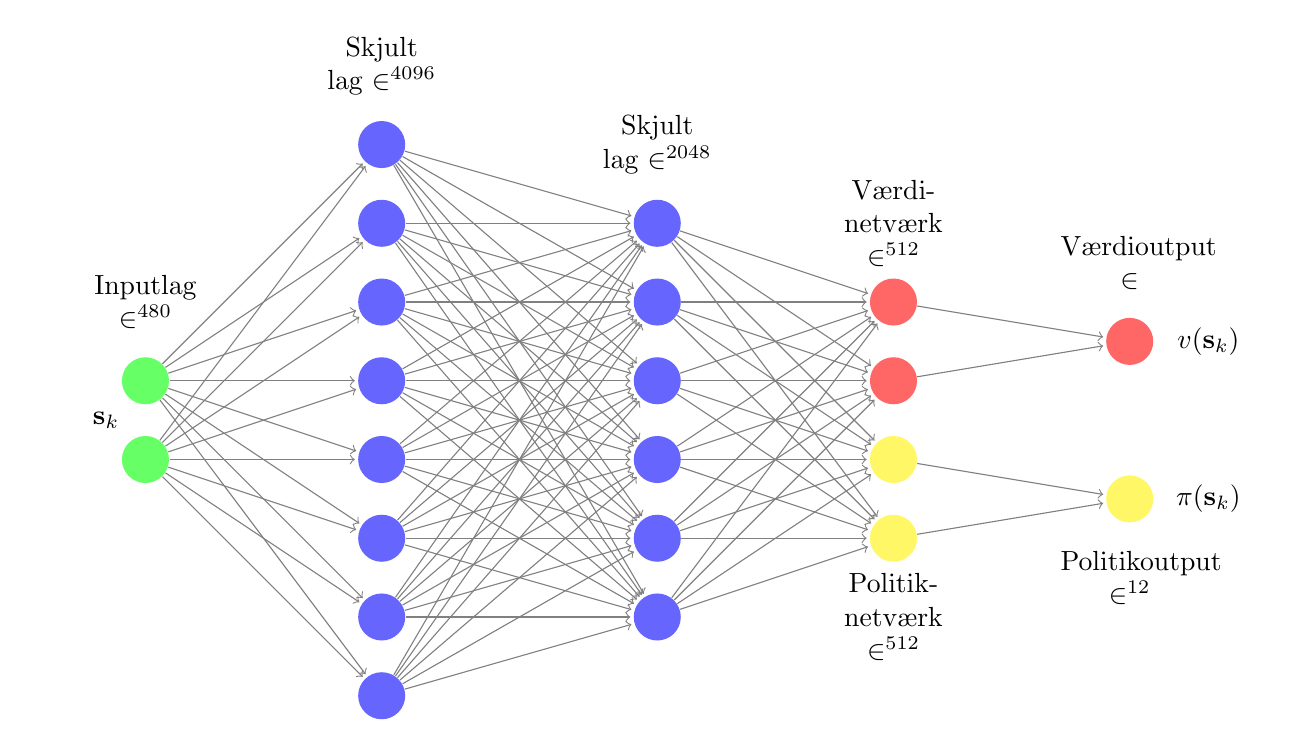
\begin{tikzpicture}[shorten >=1pt,->,draw=black!50, node distance=\layersep]
\tikzstyle{every pin edge}=[<-,shorten <=1pt]
\tikzstyle{neuron}=[circle,fill=black!25,minimum size=17pt,inner sep=0pt]

\tikzstyle{input neuron}=[neuron, fill=green!60];

\tikzstyle{shared neuron}=[neuron, fill=blue!60];
\tikzstyle{policy neuron}=[neuron, fill=yellow!60];
\tikzstyle{value neuron}=[neuron, fill=red!60];

\tikzstyle{annot} = [text width=5em, text centered]

% Draw the input layer nodes

    \foreach \name / \y in {1,...,2}
   		\path[yshift=0.5cm]
		node[input neuron] (I-\name) at (0.5,-3-\y) {};


% Draw the two hidden layers
	\foreach \name / \y in {1,...,8}
		\path[yshift=0.5cm]
			node[shared neuron] (H-\name) at (\hsep,-\y) {};
			
	\foreach \name / \y in {1,...,6}
		\path[yshift=0.5cm]
			node[shared neuron] (O-\name) at (\usep,-1-\y) {};
			
% Draw value network
	\foreach \name / \y in {1,...,2}
		\path[yshift=0.5cm]
			node[value neuron] (V-\name) at (\valsep,-2-\y) {};
			
% Draw policy network 
	\foreach \name / \y in {1,...,2}
		\path[yshift=0.5cm]
			node[policy neuron] (P-\name) at (\valsep,-4-\y) {};
% Draw value output
	\path[yshift=0.5cm]
		node[value neuron] (VO) at (\outsep, -3.5) {};
		
% Draw policy output 
	\path[yshift=0.5cm]
		node[policy neuron] (PO) at (\outsep,-5.5) {};
% Connect every layers 

    \foreach \source in {1,...,2}
		\foreach \dest in {1,...,8}
			\path (I-\source) edge (H-\dest);
			
    \foreach \source in {1,...,8}
		\foreach \dest in {1,...,6}
			\path (H-\source) edge (O-\dest);

    \foreach \source in {1,...,6}
		\foreach \dest in {1,...,2}
			\path (O-\source) edge (V-\dest);

    \foreach \source in {1,...,6}
		\foreach \dest in {1,...,2}
			\path (O-\source) edge (P-\dest);
			
	\foreach \source in {1,...,2}
		\path (V-\source) edge (VO);
		
 	\foreach \source in {1,...,2}
			\path (P-\source) edge (PO);
% Annotate the layers
\node[annot,above of=I-1, node distance=1cm]  {Inputlag \(\in \RR^{480}\)};
\node[annot,above of=H-1, node distance=1cm]  {Skjult lag \(\in \RR^{4096}\)};
\node[annot,above of=O-1, node distance=1cm]  {Skjult lag \(\in \RR^{2048}\)};
\node[annot,above of=V-1, node distance=1cm]  {Værdi-netværk \(\in \RR^{512}\)};
\node[annot,below of=P-2, node distance=1cm]  {Politik-netværk \(\in \RR^{512}\)};
\node[annot,above of=VO, node distance=1cm]  {Værdioutput \(\in \RR\)};
\node[annot,below of=PO, node distance=1cm]  {Politikoutput \(\in \RR^{12}\)};
%{Input \(\in \RR ^{288}\)};

%\node[annot,above of=H-1, node distance=1cm] (hl) {Hidden layer};

\node[annot, node distance=1cm] at (0, -4)  {\(\mathbf s_k\)};
\node[annot,right of=VO, node distance=1cm] {\(v(\mathbf s_k)\)};
\node[annot,right of=PO, node distance=1cm]  {\(\bm \pi(\mathbf s_k)\)};
\end{tikzpicture}

